\tikzset{main node/.style={circle,fill=white!20,draw,minimum size=0.5cm,inner sep=0pt},}
\usetikzlibrary{graphs,graphs.standard}

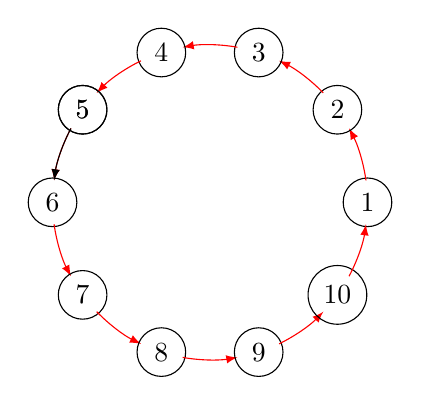
\begin{tikzpicture}

\def \n {10}
\def \radius {2cm}
\def \margin {8} % margin in angles, depends on the radius

\foreach \s in {1,...,10}
{
  \node[draw, circle] at ({360/\n * (\s - 1)}:\radius) {$\s$};
  \draw[->, >=latex, red] ({360/\n * (\s - 1)+\margin}:\radius)
    arc ({360/\n * (\s - 1)+\margin}:{360/\n * (\s)-\margin}:\radius);
}
  \node[draw, circle] at ({360/\n * (5 - 1)}:\radius) {$5$};
  \draw[->, >=latex] ({360/\n * (5 - 1)+\margin}:\radius)
    arc ({360/\n * (5 - 1)+\margin}:{360/\n * (5)-\margin}:\radius);

\end{tikzpicture}